\begin{frame}{Mesurer le degré d'intertextualité}
Mesurer informatiquement l'impact de Charcot sur son \og{}réseau\fg{} \\$\rightarrow$ intertextualité uni-directionnelle\\
\begin{itemize}
\item {\small rapports entre une œuvre et d'autres qui l'ont précédée ou suivie \\
\begin{flushright} 
(\cite{riffaterre1980trace})}
\end{flushright}
\end{itemize}
\begin{figure}[!h]
    \centering
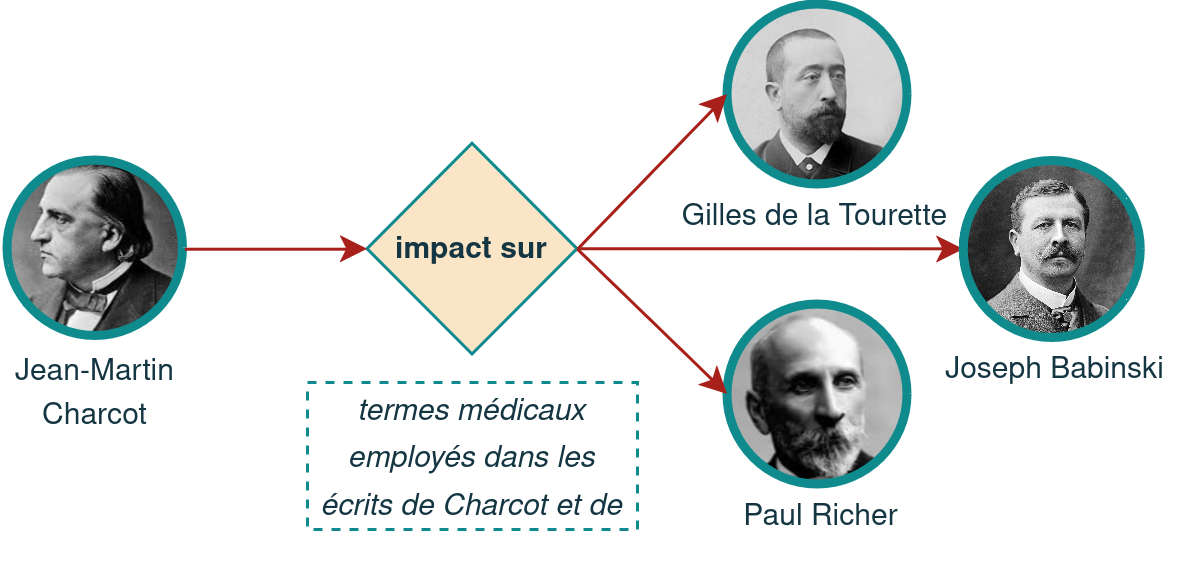
\includegraphics[width=100mm,scale=0.5]{pic/charcot_intertextualite.png}
    \caption{Opérationnalisation de l'impact de Charcot sur ses élèves.}
    \label{fig:my_label}
\end{figure}
\end{frame}

\begin{frame}{Corpus Charcot}
\begin{block}{SorbonNum\footnote{\tiny{\url{https://patrimoine.sorbonne-universite.fr/}}} | Bibliothèque de Sorbonne Université (BSU)}
201 documents XML OCRisés (sans post-correction)
\end{block}
\begin{itemize}
    \item \textrm{Charcot} : textes rédigés par Charcot
    \item \textrm{Autres} : textes rédigés par son réseau scientifique
\end{itemize}
\begin{table}[!ht]
    \centering
    \begin{tabular}{|c|c|c|}
    \hline 
    \rowcolor{gray!30}
       Corpus & Nb de docs & Nb de tokens \\
       \hline
       \textrm{Charcot}  & 68 & 12 190 649 (38,12 \%) \\
       \textrm{Autres}  & 133 & 19 788 830 (61,88 \%) \\
       \hline\hline
       \textbf{Total} & \textbf{201} & \textbf{31 979 479} (100 \%)\\
       \hline
    \end{tabular}
    \caption{Répartition du corpus issu du fonds Charcot\footnote{\tiny{\url{https://patrimoine.sorbonne-universite.fr/collection/Fonds-Charcot}}}.}
    \label{tab:my_label}
\end{table}
\end{frame}

\begin{frame}{OBVIE -- recherche textuelle, corpus Charcot\footnote{\url{https://obtic.huma-num.fr/obvie/charcot/?view=corpus}}}
\textsc{OBVIE} : moteur de recherche avancée {\small\citep{alrahabi2022obvie}}\\
{\small \danger quantification de l'importance des \og{}collocations\fg{} (\cite{nerima2006})}
\begin{figure}[!h]
    \centering
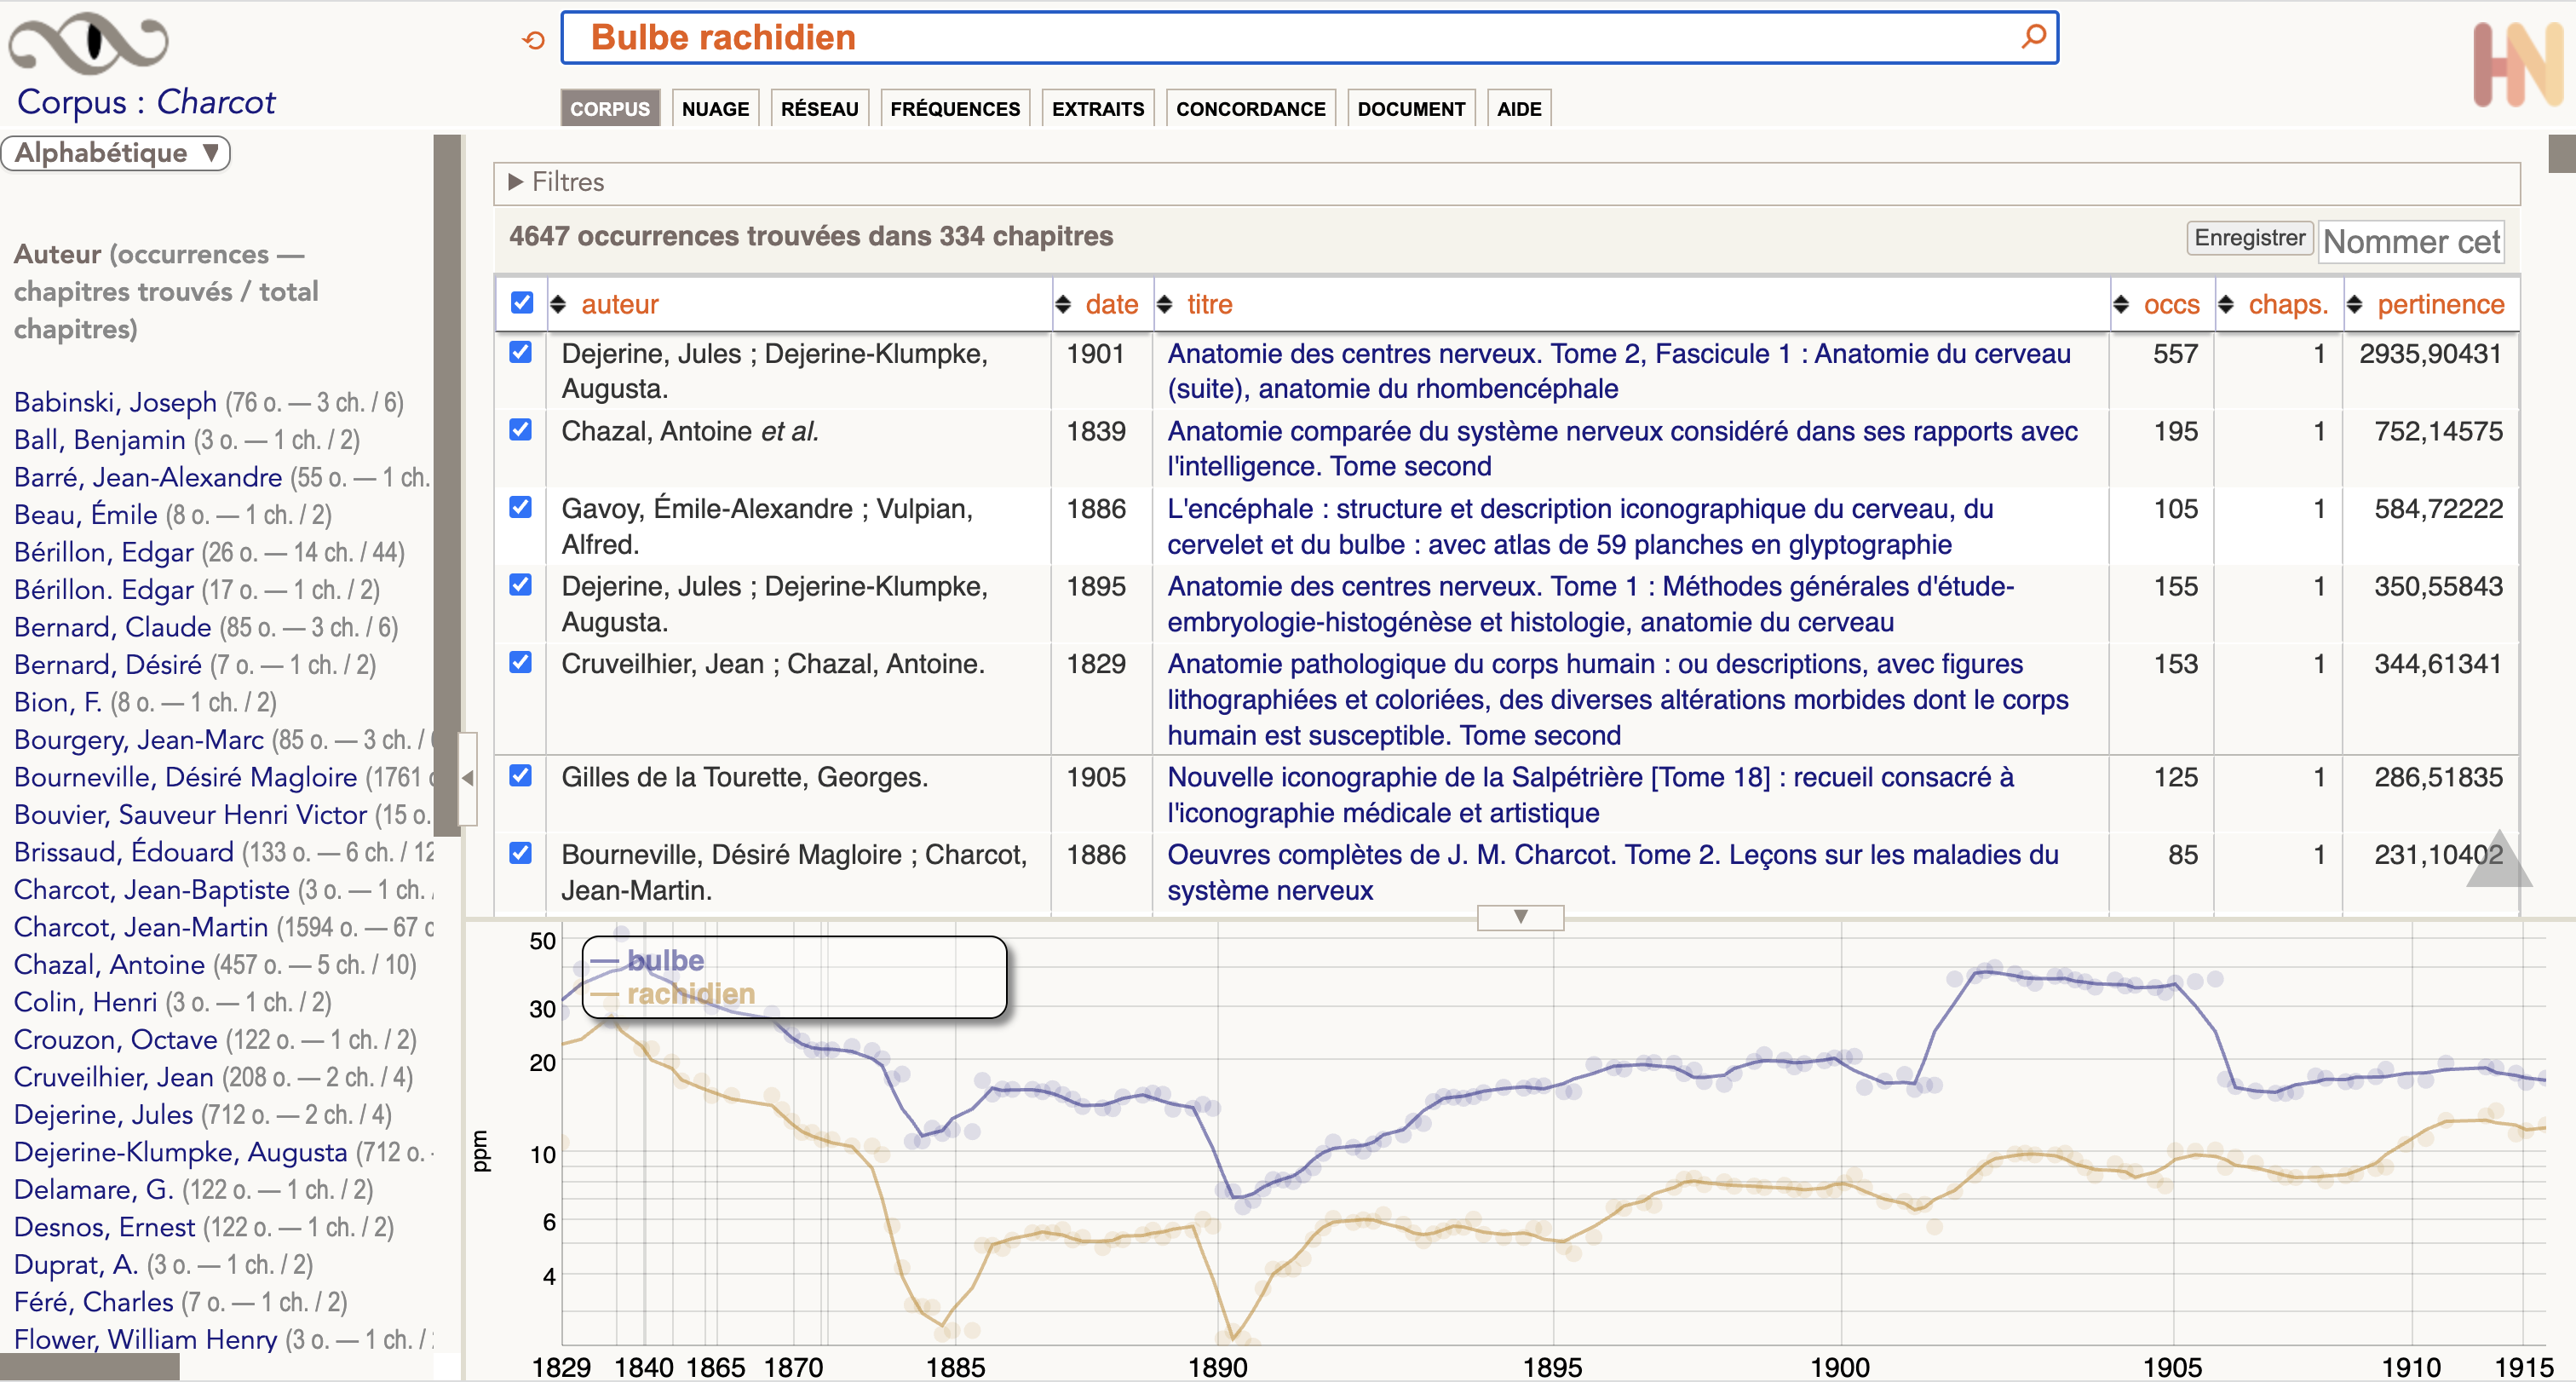
\includegraphics[width=90mm,scale=0.5]{pic/bulbe_rachidien_mini.png}
    \caption{Distribution des fréquences des tokens avec la frise chronologique pour ceux constituant l'expression \textit{bulbe rachidien} (issus des corpus \og{}Charcot\fg{} et \og{}Autres\fg{}).}
    \label{fig:my_label}
\end{figure}
% citations directes (\cite{manjavacas2019})
\end{frame}

\begin{frame}{OBVIE -- comparaison des documents similaires}
\begin{itemize}
\item fouille avancée des corpus en \textsc{XML-TEI}
\item textes similaires : mots fréquents / en commun, noms cités
\end{itemize}
%\danger impossible de quantifier l'importance des MWEs
\begin{figure}[!h]
    \centering
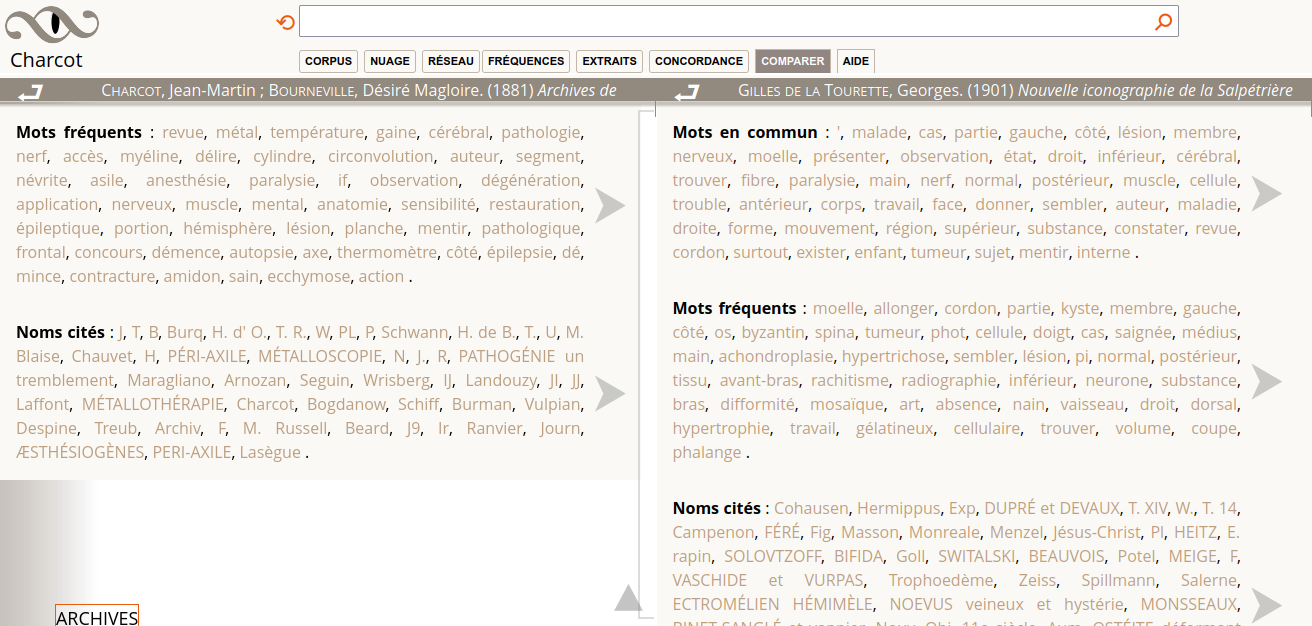
\includegraphics[width=100mm,scale=0.5]{pic/doc_sim.png}
    \caption{Points similaires entre un ouvrage de Charcot et celui de de la Tourette.}
%    \caption{Distribution des fréquences des tokens avec la frise chronologique pour ceux constituant l'expression \textit{bulbe rachidien} (issus des corpus \og{}Charcot\fg{} et \og{}Autres\fg{}).}
    \label{fig:my_label}
\end{figure}
% citations directes (\cite{manjavacas2019})
\end{frame}

\begin{frame}{TextPair -- alignement de textes, corpus Charcot\footnote{\url{https://anomander.uchicago.edu/text-pair/charcot2autres/}}}
\danger nombre de
résultats assez conséquent -- filtrage nécessaire
    \begin{figure}[!ht]
        \centering
        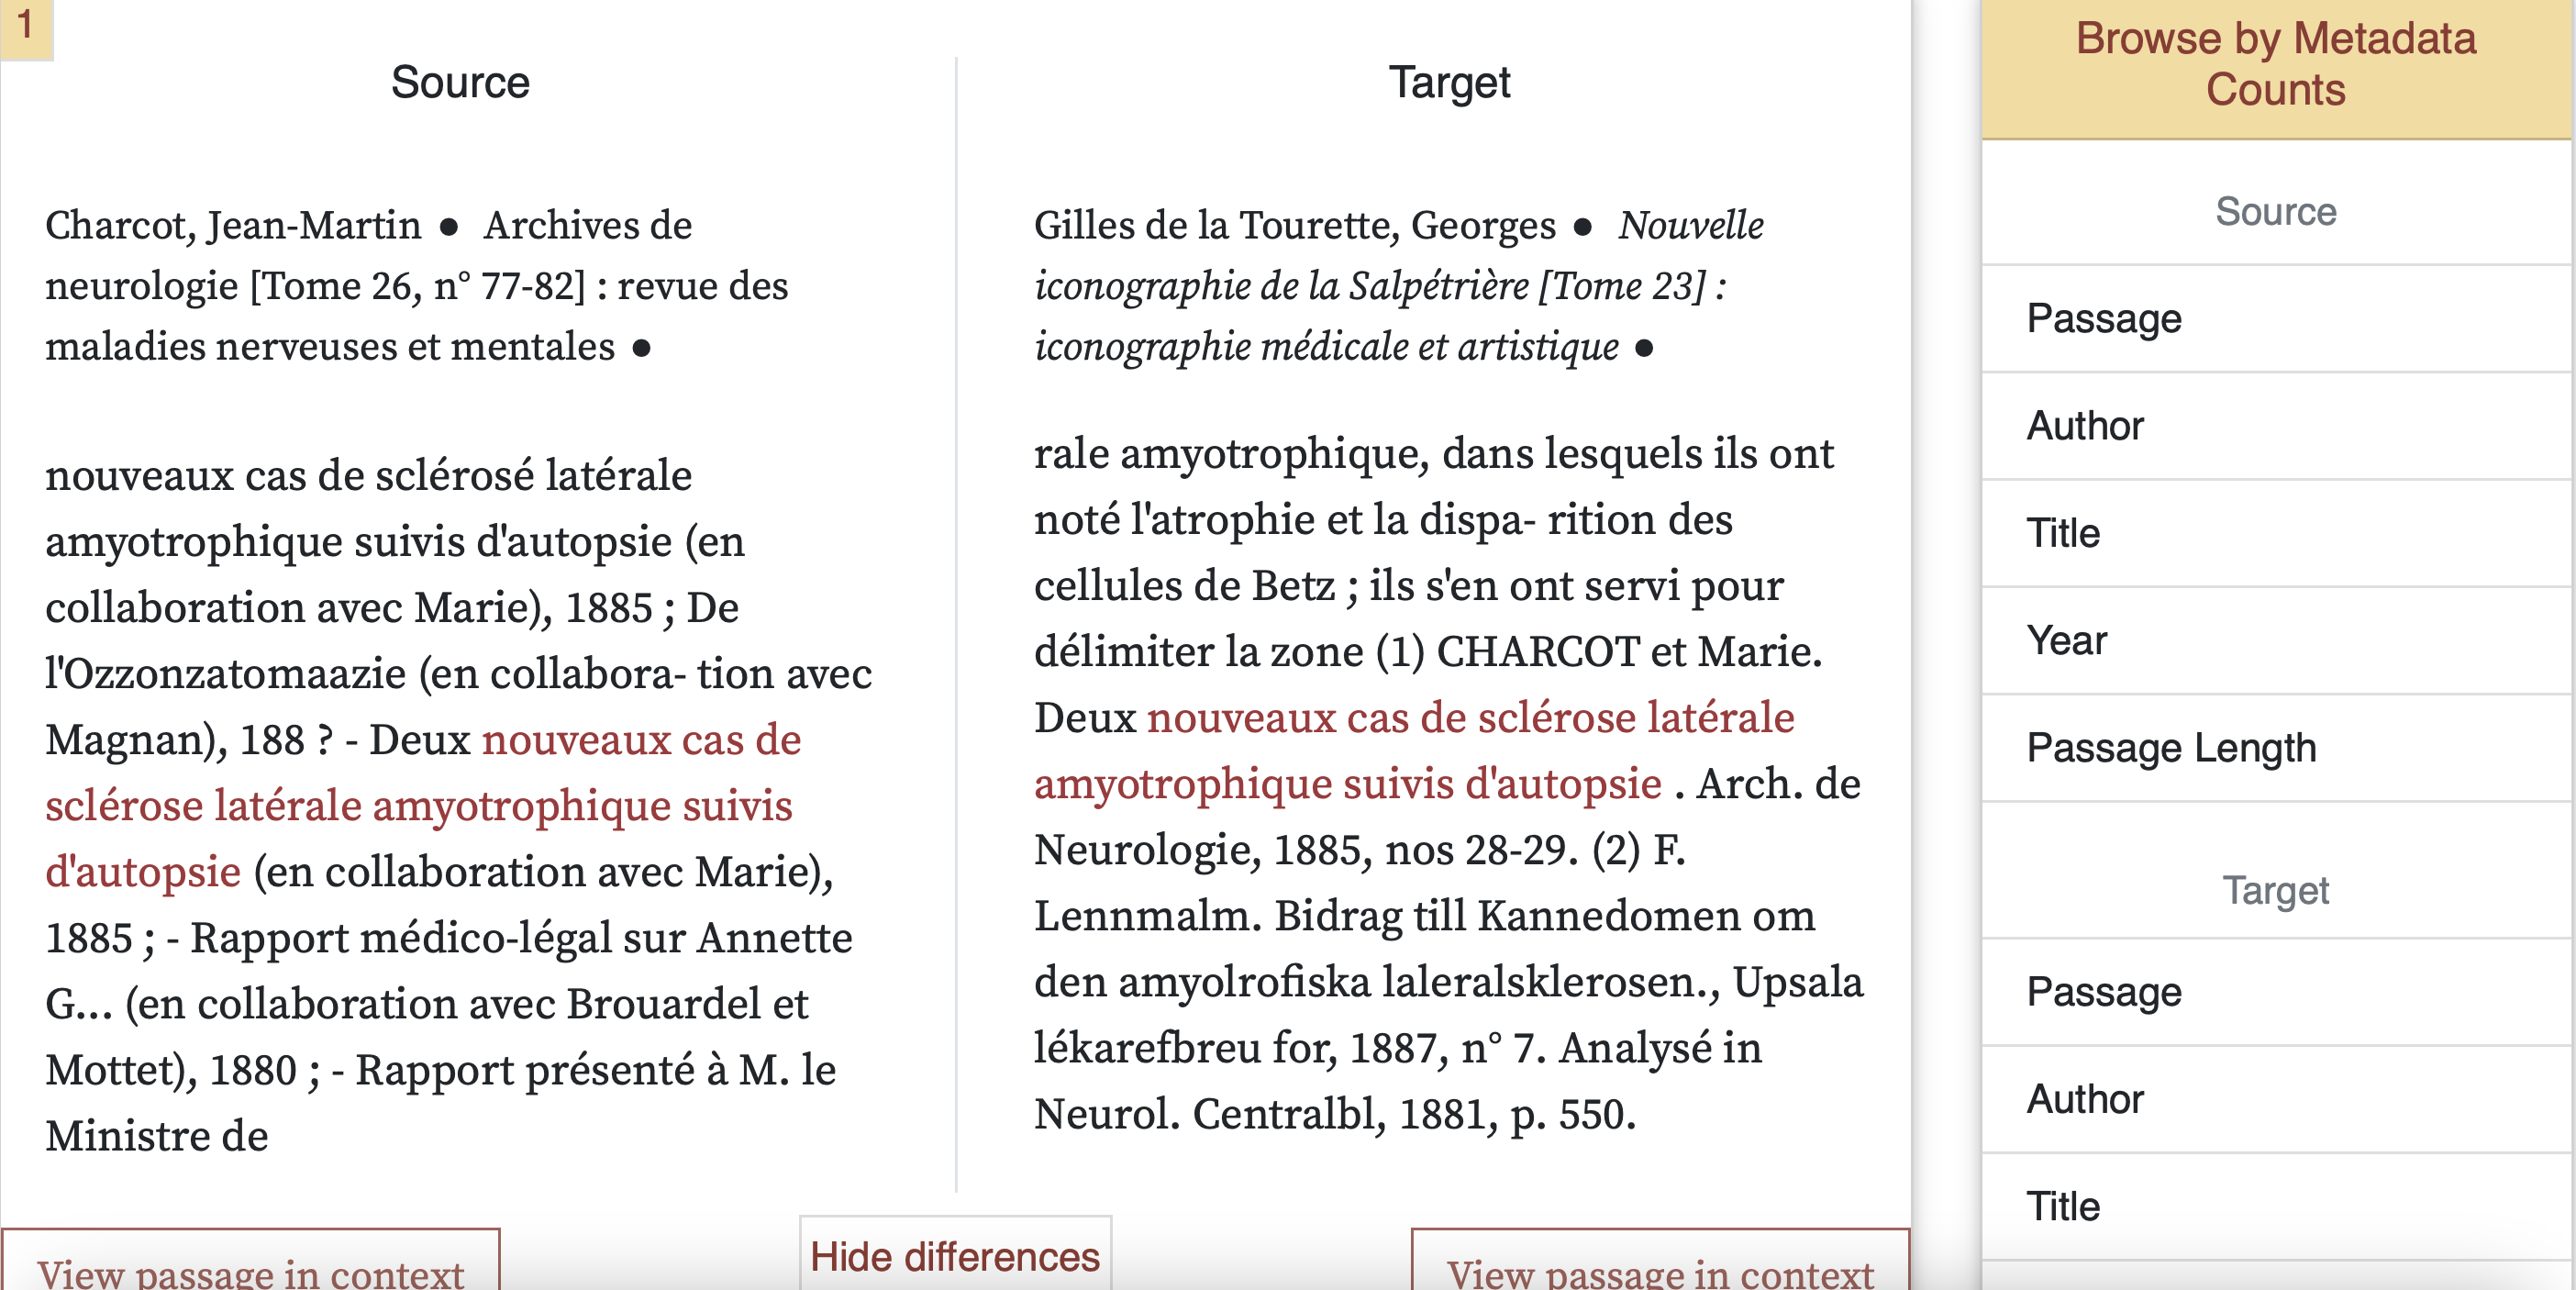
\includegraphics[width=90mm,scale=0.5]{pic/textpair.png}
        \caption{Alignement et comparaison des textes de
Charcot à celui de Georges Gilles de la Tourette (le seul
résultat) en lançant la requête \textit{sclérose latérale
amyotrophique}.}
        \label{fig:enter-label}
    \end{figure}
\end{frame}



\begin{frame}{Liste des concepts médicaux}
Extraction semi-automatique des termes en lien avec Charcot.\\~\\

 \begin{figure}[!htb]
    \centering
    \begin{minipage}{.5\textwidth}
        \centering
        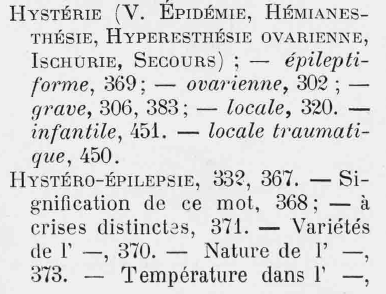
\includegraphics[width=0.6\linewidth, height=0.3\textheight]{pic/concepts-pdf}
        \caption{Index des termes \citep{charcot1890oeuvres}.}
        \label{fig:prob1_6_2}
    \end{minipage}%
    \begin{minipage}{.5\textwidth}
        \centering
        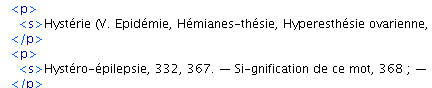
\includegraphics[width=1\linewidth, height=0.15\textheight]{pic/concepts-xml}
        \caption{Concepts médicaux, document XML.}
        \label{fig:prob1_6_1}
    \end{minipage}
\end{figure}
\begin{figure}[!htb]
    \centering
    \begin{minipage}{.5\textwidth}
        \centering
        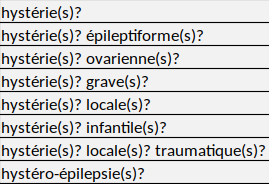
\includegraphics[width=0.6\linewidth, height=0.25\textheight]{pic/concepts-csv}
        \caption{Liste finale des concepts médicaux.}
        \label{fig:prob1_6_2}
    \end{minipage}%
    \begin{minipage}{.6\textwidth}
        \centering
   \begin{enumerate}
   \setcounter{enumi}{3}
   \item entre \texttt{<s>} et \texttt{,-(} (regex)
   \item sans termes génériques (\textit{os}, \textit{peau})
\item prise en compte des sg. / pl. (regex)
   \end{enumerate}
    \end{minipage}
\end{figure}
\end{frame}

